\documentclass[../main.tex]{subfiles}
%!TEX root = ./appendixVectoringMotor.tex
\graphicspath {{../}}

\begin{document}
\section{Vectoring Motor} \label{vectoringMotor}
In order to determine the required torque of the servo that is at the end  of the thruster shaft, worst case scenario moments of inertia were considered, as seen in Figure \ref{fig:vectoringAnalysis}. The angular acceleration can be set for any chosen servo motor as long as the acceleration is less than the specified maximum. The shaft is hollow, the thruster motor and propeller motor mounting bracket were assumed as a single rectangular prism. The propeller was also modelled as a rectangular prism. The motor torque at 7.4V is $T_{servo} = 35kg\cdot{}cm (3.4323N\cdot{}m)$, therefore the maximum angular acceleration will be $\alpha=\frac{T_{servo}}{I_{total}}$.

\begin{equation}
I_{total} = \frac{m_{shaft}\cdot{}r_{st}^2}{2} + \frac{(m_{motor} + m_{bracket})}{12} \cdot{}(d_{m_{x}}^2 + d_{m_{z}}^2) + \frac{m_{prop}}{12}\cdot{}(d_{p+{x}}^2 + d_{p_{z}}^2)
\end{equation}
\\$$ I_{total} = \frac{0.02072kg\cdot{}(0.006m)^2}{2} + \frac{(0.136kg + 0.02657kg )}{12} \cdot{}((0.03493m)^2 + (0.0381m)^2)+\frac{0.0309kg}{12}\cdot{}((0.0058m)^2 + (0.3302m)^2) $$
$$I_{total}=3.17\cdot{}10^{-4}kg\cdot{}m^2$$
$$\alpha=\frac{T_{servo}}{I_{total}}=\frac{3.4323N\cdot{}m}{3.17\cdot{}10^{-4}kg\cdot{}m^2}$$
$$\alpha=10827rad/s^2$$

Ideally, we would have perfectly balanced the motor on the shaft so that the moments of inertia about the rotation axis of the shaft equalled zero. However, it is still clear by the calculation shown that the inertia is very low and the servo will most likely not need to hold the position of the thruster.

\begin{figure}[H]
	\centering
	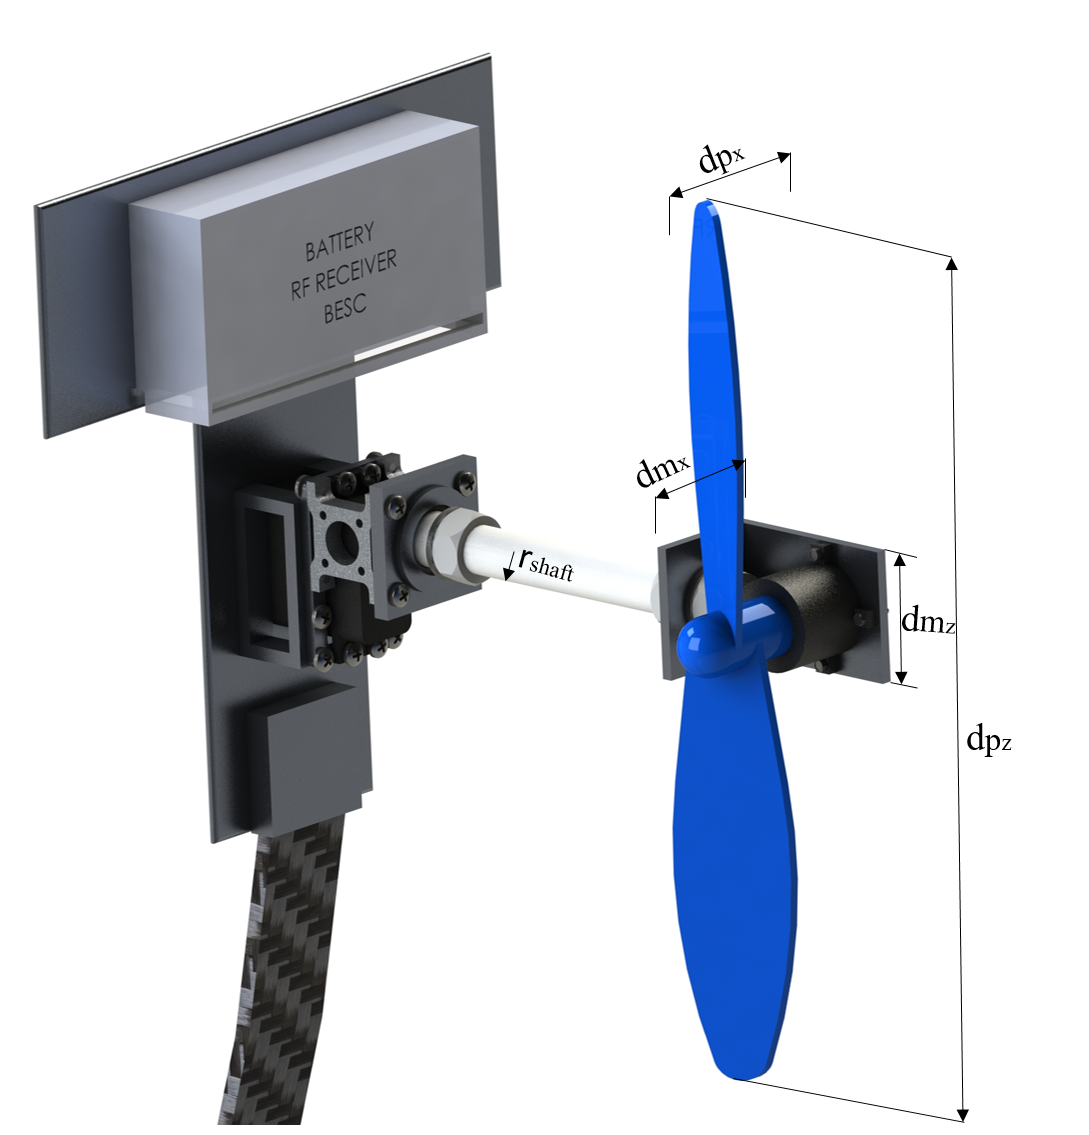
\includegraphics[width=0.5\textwidth]{img/analysis/thrusterTorque/vectoringAnalysis.png}
	\caption{Thruster Pitching Shaft Worst Case Moment of Inertia}
	\label{fig:vectoringAnalysis}
\end{figure}

\end{document}